\documentclass[sigplan,nonacm]{acmart}
\usepackage{booktabs}
\setlength{\emergencystretch}{2em}
\settopmatter{printacmref=false,printccs=false,printfolios=true}
\setcopyright{none}
\renewcommand\footnotetextcopyrightpermission[1]{}
\title{Mini-Paper 2: Symbolic Regression}
\author{Carleano Chang}
\email{poching2@illinois.edu}
\affiliation{\institution{University of Illinois Urbana-Champaign}\city{Urbana}\state{Illinois}\country{USA}}
\author{Christine Liou}
\email{ycliou2@illinois.edu}
\affiliation{\institution{University of Illinois Urbana-Champaign}\city{Urbana}\state{Illinois}\country{USA}}
\begin{document}
\begin{abstract}
We improve a C++ symbolic regression program using compiler optimization, direct stack indexing, and sorting with fewer program copies. We measure three CSV datasets and two image workloads with unchanged search settings. The final version is 12.60 times faster on Diabetes, 9.74 times on Cancer, 10.03 times on Housing, 11.05 times on Silk waves, and 10.95 times on Square waves. Emitted formulas and printed quality metrics match the baseline; reconstructed PNGs also match. Separate memory and integer-overflow fixes pass the recorded correctness checks.
\end{abstract}
\maketitle
\noindent\textbf{Code Repository:} \url{https://github.com/Car1eano/fall26-cs598ape-mp2}

\section{Approach and Baseline}
The supplied program searches for mathematical expressions using genetic programming~\cite{starter}. Candidate expressions are trees. Tournament selection chooses parents, and crossover and mutation produce new candidates. Evaluating these candidates on training rows gives their fitness. Diabetes and Housing use regression, while Cancer uses classification with log loss and a sigmoid output. The image benchmarks learn expressions from pixel coordinates to RGB values.

We use the original commit \texttt{f19cc63} as the baseline. All performance measurements use the same course VM: four Intel Xeon Silver 4216 vCPUs, about 16 GiB RAM, Ubuntu 26.04.1, and G++ 15.2.0. The original C++17 build has no optimization-level flag. We test \texttt{-O2} separately and with source changes; other build flags are unchanged. We do not add \texttt{-ffast-math} or machine-specific instructions.

Diabetes has 442 rows and 10 features; Housing has 20,640 rows and 8 features. Both use population 512, up to 16 generations, tournament size 4, and seed 2025000000. Cancer has 569 rows and 30 features, population 16,384, up to 16 generations, tournament size 16, and seed 2025. The original deterministic split reserves about 20\% for testing. Function sets, stopping criteria, and data remain unchanged.

Both images are $256\times256$ RGB inputs. Each model uses 128 candidates, 16 generations, tournament size 4, and disabled early stopping. Silk averages three models per channel (nine total); Square averages eight (24 total). Coordinates are mapped to $[-\pi,\pi]$. Model seeds are $2025000000+cK+m$, for channel $c$ and model $m$.

Each configuration has one warmup and three measured runs. We use median internal time and divide baseline by optimized medians for speedup. There are 100 runs: seven stages on three CSV datasets and two stages on each image. Warmups account for 25 runs. The supplied timer covers loading, preparation, training, testing, and formula output, but stops before final local cleanup. External process times are also saved. Racket PNG rendering is measured separately and excluded from speedups.

\section{Optimizations and Fixes}
\subsection{Compiler Optimization and Stack Indexing}
\texttt{-O2} is a build optimization~\cite{gcc}. It changes how the existing C++ is compiled without changing search settings. Independently, it reduces Diabetes time from 21.220 to 10.170 seconds, Cancer from 130.977 to 60.702 seconds, and Housing from 248.850 to 117.940 seconds.

Hardware profiling with \texttt{perf} was blocked by VM permissions. We therefore used \texttt{gprof} with \texttt{-pg}~\cite{gprof}. In the original Diabetes profile, stack push accounts for 46.11\% of self time and pop for 6.67\%, with 227,521,496 calls to each. These instrumented percentages motivate the change; they are not uninstrumented runtime estimates.

The original fixed-capacity stack scans slots during push and pop. In \path{src/reg_stack.h}, we replace these scans with indexing through the current element count. Push writes to the next slot; pop decrements the count and reads that slot. This is a data-structure implementation and work-reduction change. It preserves last-in-first-out order, ignores pushes to a full stack, and returns zero on an empty pop. It applies to the shared expression evaluator and assumes the existing count/capacity invariant.

Stack indexing alone gives speedups of 2.49, 1.84, and 2.21 on Diabetes, Cancer, and Housing. Together with \texttt{-O2}, the times become 1.717, 18.293, and 24.913 seconds. The combined benefit is larger than either change alone. Simpler indexing may help compiler optimization, but we did not verify the specific mechanism in assembly.

\subsection{Sorting with Fewer Copies}
After the stack and compiler changes, the Cancer profile shows insertion sorting at about 29.5\% cumulative time. Assigning a program deep-copies its expression nodes, making repeated object movement costly for the 16,384-candidate population.

In \path{benchmark/genetic_benchmark.cpp}, we stable-sort integer indices by fitness, build an ordered snapshot, and copy it back. Stable ordering preserves the original order of equal-fitness candidates. The original handling of NaN fitness values is retained. The snapshot keeps all sources alive during reordering, at the cost of extra temporary storage. This applies to the benchmark's ranking step, rather than changing genetic selection or reducing the search budget.

In the Cancer profiles, total program assignments fall from 65,190,213 to 329,285. Node-evaluation calls remain 1,353,683,384. Measured Cancer time falls from 18.293 to 13.292 seconds, an additional 1.38 times speedup. Diabetes and Housing change only slightly. These workloads have much smaller populations, consistent with less sorting work.

\subsection{Memory and Integer-Range Fixes}
Hoist mutation replaced a reused output object's node array without freeing the previous array. In \path{src/program.cpp}, we allocate and copy the replacement before deleting the old nodes. Original Diabetes Valgrind reports 58,776 bytes in 91 definitely lost blocks; final Diabetes reports zero errors and no heap bytes in use at exit~\cite{valgrind}.

UBSan also found signed overflow in the custom integer distribution's range-size arithmetic. We widen operands before subtraction and addition in \path{include/custom_distributions.h}, keeping rejection sampling. Tests check random sequences and engine consumption for the tested ranges. This does not establish equivalence for every case of the original undefined behavior. These two changes are correctness fixes; their small timing differences do not establish further speedups.

\begin{figure}[t]
\centering
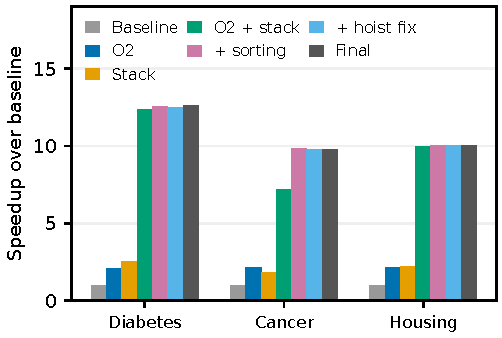
\includegraphics[width=\columnwidth]{figures/stages.pdf}
\caption{CSV speedups using median internal times. Sorting and hoist stages include prior changes; final also includes the integer-range fix. O2 and stack were additionally measured independently.}
\label{fig:stages}
\end{figure}

\section{Evaluation and Correctness}
Figure~\ref{fig:stages} compares all seven CSV stages. Figure~\ref{fig:overview} and Table~\ref{tab:times} show the baseline/final comparison for all five workloads. Images were measured only at these two stages, so we cannot assign their speedups to individual changes.

\begin{table}[t]
\caption{Median internal time in seconds. Three measured runs per entry; warmups excluded.}
\label{tab:times}
\centering
\begin{tabular}{lrrr}
\toprule
Workload & Baseline & Final & Speedup \\
\midrule
Diabetes & 21.220 & 1.684 & 12.60$\times$ \\
Cancer & 130.977 & 13.449 & 9.74$\times$ \\
Housing & 248.850 & 24.809 & 10.03$\times$ \\
Silk waves & 426.405 & 38.586 & 11.05$\times$ \\
Square waves & 1319.584 & 120.481 & 10.95$\times$ \\
\bottomrule
\end{tabular}
\end{table}

Saved summaries include min--max, mean, and sample standard deviation. For example, baseline Silk ranges from 411.229 to 427.364 seconds; final Silk ranges from 38.552 to 38.846 seconds. Baseline Square ranges from 1275.788 to 1319.917 seconds; final Square ranges from 120.273 to 120.554 seconds. Three repeats describe observed timing variation, not statistical significance. Fixed-seed repeats do not measure quality variation across seeds. Runs use a shared VM without CPU affinity, and batches were not interleaved.

After removing timing lines, emitted formulas and printed metrics match baseline for all recorded stages. For example, Diabetes test MSE values remain 7468.95 and 7217.17 for the two exported formulas; Cancer accuracy remains 0.946903. Housing test MSE values remain 0.64586 and 0.728984. RGB test MSE before display clamping remains 0.0277195631 for Silk and 0.0175210362 for Square. All eight reconstructed PNGs per image have matching hashes across baseline and final runs. Neither reconstruction exactly matches its input: speed improved while quality was preserved. Matching outputs do not prove that every intermediate training state is identical.

Full-workload AddressSanitizer and UndefinedBehaviorSanitizer checks, with leak detection, pass for all five final workloads. Full Valgrind was run for Diabetes only. Unit checks cover stack boundaries, 1,000 expression trees against a recursive evaluator, stable sorting including NaNs and ties, repeated hoist mutation, and integer-distribution behavior. Seventeen Python tests validate benchmark tools and rejection of inconsistent records.

For reproducibility, a clean local clone and new Python environment ran all five workloads once per version. Formulas, quality records, and PNGs matched saved results; statistics and figures regenerated. These ten single runs are verification only, not performance samples. System packages were shared with the existing VM, so this was not a fresh-OS installation test. The README records packages, commands, flags, and stage commits.

\begin{figure}[t]
\centering
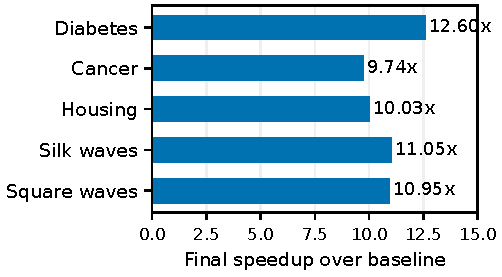
\includegraphics[width=\columnwidth]{figures/overview.pdf}
\caption{Final speedup on all five workloads. Each value is the ratio of baseline and final median internal times. PNG rendering and diagnostic runs are excluded.}
\label{fig:overview}
\end{figure}

\section{Introspection}
The largest gains came from removing repeated stack work and enabling compiler optimization. Once these costs fell, Cancer's copying during sorting became a useful next target. Its much larger population explains why the ranking change matters more there than on the other CSV cases. This supports profiling again after each substantial change, rather than assuming the first bottleneck remains dominant.

Stable sorting requires extra index and expression storage; peak memory was not measured. We did not test parallelism, SIMD, or \texttt{-O3}. They remain possible extensions, but the current evidence does not establish their benefit. Instrumented profiles explain candidate bottlenecks; all speedups come from separate uninstrumented runs.

\section{Teamwork}
Carleano focused on the O2 and stack changes, the integer-range fix, CSV results, and build and benchmark commands. Christine focused on sorting, hoist memory cleanup, image reconstruction, and correctness and memory evidence. We used driver and observer roles to discuss the changes and check results. Both members reviewed and approved the five changes, connecting implementation decisions with performance and correctness evidence.

\section{Conclusion}
Compiler optimization, direct stack indexing, and reduced copying make the five fixed workloads 9.74 to 12.60 times faster. Memory and overflow fixes address separate correctness issues. Saved formulas, printed metrics, and reconstructed PNGs remain unchanged under the tested settings, with reproducible commands and raw evidence retained in the artifact.

\newpage
\begin{thebibliography}{4}
\bibitem{starter} PRONTOLab. 2026. CS598APE Homework 2 starter code and assignment. \url{https://github.com/PRONTOLab/598APE-HW2}.
\bibitem{gcc} Free Software Foundation. GCC 15.2: Options That Control Optimization. \url{https://gcc.gnu.org/onlinedocs/gcc-15.2.0/gcc/Optimize-Options.html}.
\bibitem{gprof} Free Software Foundation. GNU gprof Manual. \url{https://sourceware.org/binutils/docs/gprof/}.
\bibitem{valgrind} Valgrind Developers. Memcheck: a Memory Error Detector. \url{https://valgrind.org/docs/manual/mc-manual.html}.
\end{thebibliography}
\end{document}
